\documentclass{article}

\usepackage{url}
\usepackage{amsmath,amssymb}
\usepackage{setspace}
\usepackage{verbatim}
% \usepackage{subfig} %subfigure
\usepackage{graphicx} %subfigure
\usepackage{caption} % subfigure
\usepackage{subcaption}  %subfigure
\usepackage{listings}
\usepackage[usenames,dvipsnames]{color}
\usepackage[margin=.8in]{geometry}
\usepackage{indentfirst}
\setlength{\parindent}{0mm}
\setlength{\parskip}{0mm}
\usepackage{multirow}
\usepackage{placeins}

\title{STA 250, Lab 4}
\author{Longphi Nguyen\\ \\}
\setcounter{secnumdepth}{0}

\begin{document}
\maketitle
\section{Problem 1}

\begin{figure}
\center
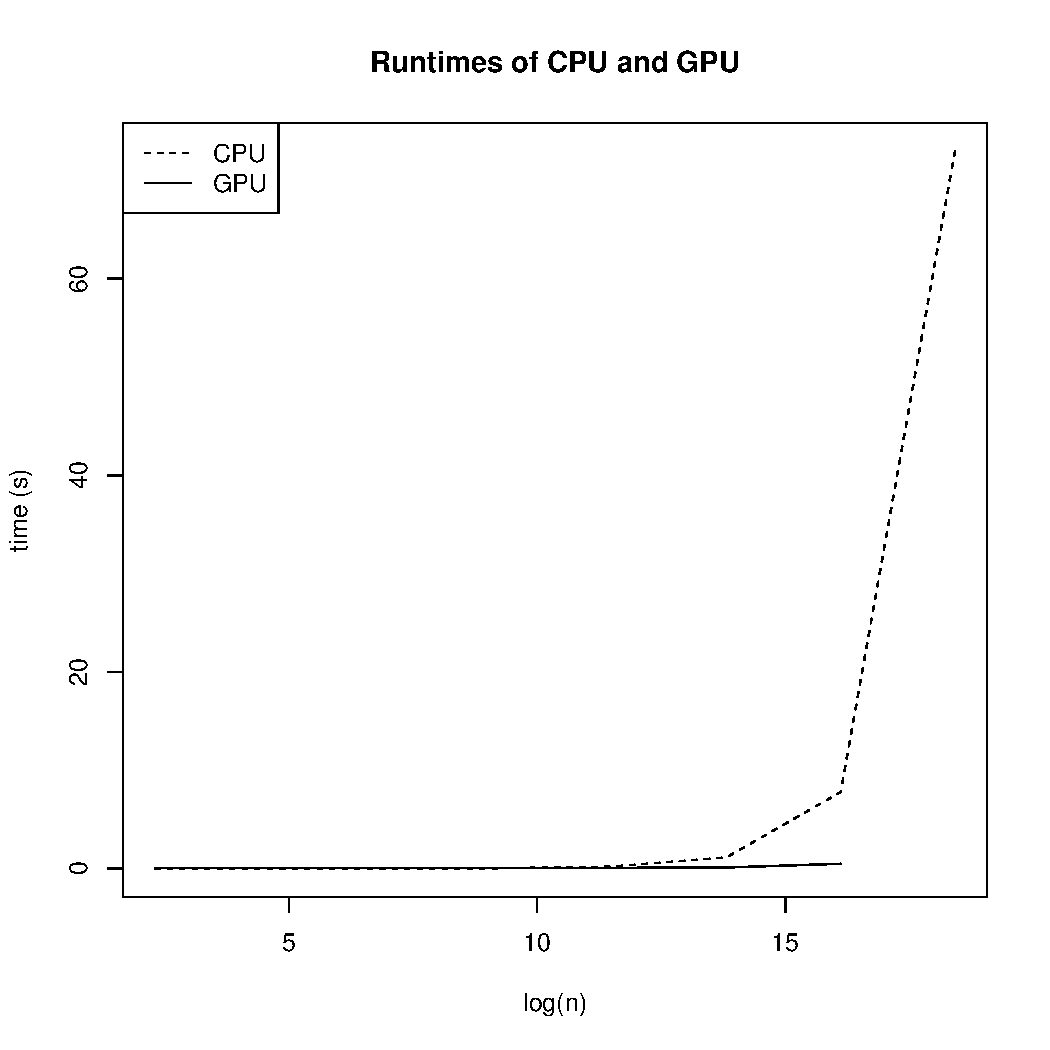
\includegraphics[width=.6\textwidth]{Q1Plot.pdf}
\caption{CPU/GPU Truncated Normal sampling computation times}
\label{fig1}
\end{figure}

From Figure \eqref{fig1}, the GPU sampling starts to outperform the CPU sampling at about $n=e^{10}\approx 22,026.$ However, the GPU code used recycling, which was convenient in this case since $\mu, \Sigma, a,$ and $b$ can be represented by 1 number. As such, not much time was needed for copying to the GPU.

\begin{center}
  \begin{tabular}{ |l | c |r| rrr| }
    \hline
n & CPU & GPU total & copyToDevice & kernel & copyFromDevice\\
\hline
$10^1$ & 0 & 0.044 & 0.004 & 0.04 & 0.00 \\
$10^2$ & 0 & 0.040 & 0.004 & 0.036 & 0.00 \\
$10^3$ & 0 & 0.040 & 0.004 & 0.036 & 0.00 \\
$10^4$ & 0.008 & 0.040 & 0.004 & 0.036 & 0.00 \\
$10^5$ & 0.18 & 0.048 & 0.004 & 0.044 & 0.00 \\
$10^6$ & 1.116 & 0.084 & 0.012 & 0.068 & 0.004 \\
$10^7$ & 7.76 & 0.464 & .064 & 0.352 & 0.048 \\
$10^8$ & 72.933 & -- & -- & -- & --\\
    \hline
  \end{tabular}
\end{center}

\section{Problem 2}

\begin{align}
P(z_i | y_i=1, \beta) &= \frac{\phi(z_i-x_i'\beta)}{\Phi(b-x_i'\beta)-\Phi(a-x_i'\beta)} \\
 &\propto \phi(z_i-x_i'\beta) = \frac{1}{\sqrt{2\pi}}e^{-\frac{1}{2}(z_i-x_i'\beta)}\\ 
 & \propto e^{-\frac{1}{2}(z_i-x_i'\beta)^2}
\end{align}

Similarly, $P(z_i | y_i=0, \beta) \propto e^{-\frac{1}{2}(z_i-x_i'\beta)^2}$
So that 
\begin{align*}
P(Z|Y, \beta) &= \prod_{i=1}^n P(z_i | y_i, \beta)\\
& \propto  e^{-\frac{1}{2}\Sigma_{i=1}^n (z_i-x_i'\beta)^2}\\
& = e^{-\frac{1}{2}(Z-X\beta)'(Z-X\beta)}
\end{align*}

where $X=[x_1, x_2, ..., x_n]'.$

Then,
\begin{align*}
P(\beta, Z | Y) &\propto P(\beta)P(Z|Y,\beta)\\ 
&\propto e^{-\frac{1}{2}[(Z-XB)'(Z-XB) - \frac{1}{2}(\beta-\beta_0)'\Sigma_0^{-1}(\beta-\beta_0)]}\\
&= e^{-\frac{1}{2}[(Z'-\beta'X')(Z-X\beta) + (\beta'\Sigma_0^{-1}-\beta_0'\Sigma_0^{-1})(\beta-\beta_0)]}\\
&= e^{-\frac{1}{2}[Z'Z + \beta'X'X\beta - Z'X\beta - \beta'X'Z + \beta' \Sigma_0^{-1}\beta - \beta'\Sigma_0^{-1}\beta_0 - \beta_0'\Sigma_0^{-1}\beta + \beta_0' \Sigma_0^{-1}\beta_0]}\\
&=e^{-\frac{1}{2}[Z'Z + \beta'(X'X + \Sigma_0^{-1})\beta - \beta'(X'Z+\Sigma_0^{-1}\beta_0) - (Z'X + \beta_0'\Sigma_0^{-1})\beta + \beta_0'\Sigma_0^{-1}\beta_0]}
\end{align*}

Marginalizing out Z and ignoring constants gives:
$$P(\beta|Z,Y) \propto e^{-\frac{1}{2}[\beta'(X'X + \Sigma_0^{-1})\beta - \beta'(X'Z+\Sigma_0^{-1}\beta_0) - (Z'X + \beta_0'\Sigma_0^{-1})\beta]}$$

This has the form of a multivariate Normal pdf, such that:

$$\beta|Z,Y \sim N((X'X+\Sigma_0^{-1})^{-1}(X'Z+\Sigma_0^{-1}\beta_0), (X'X+\Sigma_0^{-1})^{-1})$$

Then, the probit MCMC is done as follows:
\begin{enumerate}
\item Sample $z_i^{(t)}$ from an upper truncated normal if $y_i=1$ or from a lower truncated normal if $y_i=0$. Let $Z^{(t)}=[z_1^{(t)}, ..., z_n^{(t)}]'.$
\item Sample $\beta^(t)$ from $N((X'X+\Sigma_0^{-1})^{-1}(X'Z^{(t)}+\Sigma_0^{-1}\beta_0), (X'X+\Sigma_0^{-1})^{-1}).$
\end{enumerate}

\begin{figure}
\center
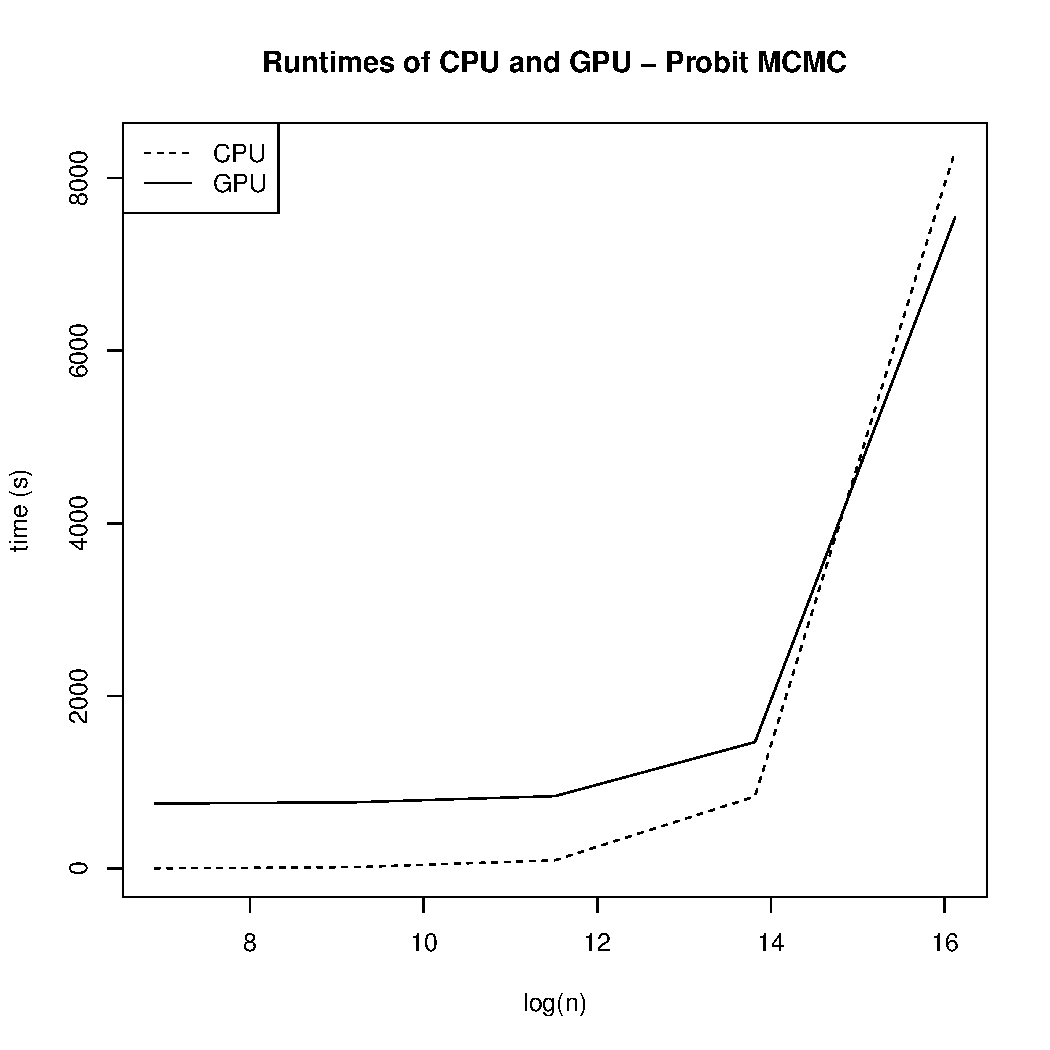
\includegraphics[width=.6\textwidth]{Q2Plot.pdf}
\caption{CPU/GPU probit MCMC computation times}
\label{fig2}
\end{figure}

\begin{center}
  \begin{tabular}{ |l | c | r| }
    \hline
n & CPU & GPU total\\ \hline
$10^3$ & 2.284 & 752.443\\
$10^4$ & 16.185 & 767.524\\
$10^5$ & 96.59 & 839.145\\
$10^6$ & 834.416 & 1464.539\\
$10^7$ & 8304.839 & 7540.419\\
    \hline
  \end{tabular}
\end{center}

From Figure \eqref{fig2}, the GPU becomes preferred at about $n=e^{15} = 3,269,017$. At that point, the CPU was not able to do the sampling as well as the GPU (though the overall time was still slow). Unlike in Problem 1, the vectors were not recycled, so the drastic difference compared to Problem 1 is expected to be from copying the large vectors to the GPU.

\section{Code (kernel.cu)}

\begin{verbatim}
#include <stdio.h>                                                              
#include <stdlib.h>                                                             
#include <cuda.h>                                                               
#include <curand_kernel.h>                                                      
#include <math_constants.h>                                                     
                                                                                
extern "C"                                                                      
{                                                                               
                                                                                
__global__ void                                                                 
rtruncnorm_kernel(float *x, int n,                                              
                  float *mu, float *sigma,                                      
                  float *a, float *b,                                           
                  int len_mu, int len_sigma,                                    
                  int len_a, int len_b,                                         
                  int maxRejections,                                            
                  int rng_c)                                                    
{                                                                               
        int rng_a=1; // These can easily be made as argument, but I'm lazy.     
        int rng_b=2;                                                            
                                                                                
        // Usual block/thread indexing...                                       
        int myblock = blockIdx.x + blockIdx.y * gridDim.x;                      
        int blocksize = blockDim.x * blockDim.y * blockDim.z;                   
        int subthread = threadIdx.z*(blockDim.x * blockDim.y) + threadIdx.y*blockDim.x + threadIdx.x;
        int idx = myblock * blocksize + subthread;                              
                                                                                
        // Determine indexes for vectors if using recycling.                    
        // Note: A good programmer would avoid the code repitions.              
        int ind_mu = ((len_mu<2) ? 0 : (idx % len_mu));                         
        int ind_sigma = ((len_sigma<2) ? 0 : (idx % len_sigma));                
        int ind_a = ((len_a<2) ? 0 : (idx % len_a));                            
        int ind_b = ((len_b<2) ? 0 : (idx % len_b));                            
                                                                                
        if (idx < n){                                                           
                // Set up RNG                                                   
                curandState rng;                                                
                curand_init(rng_a+idx*rng_b, rng_c, 0, &rng);                   
                                                                                
                // Sample truncated normal, doing rejection-sampling            
                for(int i=0; i<maxRejections; i++)                              
                {                                                               
                        float samp=mu[ind_mu]+sigma[ind_sigma]*curand_normal(&rng);
                        if(a[ind_a]<=samp && samp<=b[ind_b])                    
                        {                                                       
                                x[idx]=samp;                                    
                                return;                                         
                        }                                                       
                }                                                               
                // Could not sample using rejection-sampling.                   
                // Simply sample from Uniform(a,b).                             
                x[idx]=curand_uniform(&rng)*(a[ind_a]-b[ind_b])+a[ind_a];       
        }                                                                       
        return;                                                                 
}                                     
                                                                                
} // END extern "C" 
\end{verbatim}

\section{Code (rcuda.R)}

\begin{verbatim}
# Sample from TruncatedNorm(mu, sigma; [a,b]), trying the naive
# approach up to maxRejection times. Uses CPU.
truncnormCPU<-function(N,mu,sigma,a,b,maxRejection)
{
        # A counter. Stops rejection-sampling when sampleCount==maxRejection
        sampleCount=0
        x=rnorm(N, mu, sigma) # randomly sample from Normal
        # resample has indexes for which x is not in [a,b].
        # Then, x[resample] needs to be resampled.
        resample=which(x<a | x>b)

        while(length(resample)>0 && sampleCount<maxRejection)
        {
                x[resample]=rnorm(length(resample), mu[resample], sigma[resample])
                # Below: Find the index for which x is not in [a,b] again,
                # but we only need to check the ones that were resampled.
                resample.tmp=which(x[resample]<a[resample] | x[resample]>b[resample])
                # resample.tmp lists indexes of x.subset that needs to be
                # changed. Now, we get the actual index needed to be changed for x.
                resample=resample[resample.tmp]
                sampleCount=sampleCount+1
        }

        # If the max number of tries failed, then just sample from a uniform.
        if(length(resample)>0)
        {
                # runif does not work on Inf, so replace -Inf/Inf with min/max number for R
                a[resample][which(is.infinite(a[resample])==TRUE)]=.Machine$double.xmin
                b[resample][which(is.infinite(b[resample])==TRUE)]=.Machine$double.xmax
                x[resample]=runif(length(resample), a[resample], b[resample])
        }

        invisible(x) # Returns x
}

# This is used for sampling using Robert's suggested sampling.
# Note: Not used, because I didn't code one for the kernel, so I didn't want to be comparing
# two codes that potentially did different things.
truncnormCPU_Robert<-function(N,mu,sigma,a,b,maxRejection)
{
        sampleCount=0 # A counter. Stops rejection-sampling when sampleCount==maxRejection
        sign.a=ifelse(a>=0, 1, -1)
        a=abs(a)
        sign.b=ifelse(b>=0, 1, -1)
        b=abs(b)
        alpha=a+sqrt(a^2+4)/2

        z=rexp(N, alpha)
        g=exp(-(z-alpha)^2/2)
        u=runif(N)
        resample=which(g>u) # Has indexes for which x is not in [a,b]. Then, x[resample] needs to be resampled.

        while(length(resample)>0 && sampleCount<maxRejection)
        {
                x[resample]=rexp(length(resample), alpha[resample])
# Below: Find the index for which x is not in [a,b] again, but we only need to check the ones that were resampled.
                g=exp(-(x[resample]-alpha[resample])^2/2)
                u=runif(length(resample))
                resample.tmp=which(g>u)
                resample=resample[resample.tmp] # resample.tmp lists indexes of x.subset that needs to be changed. Now, we get the actual index needed to be changed for x.
                sampleCount=sampleCount+1
        }

# If the max number of tries failed, then just sample from a uniform.
        if(length(resample)>0)
        {
                x[resample]=runif(length(resample), a[resample], b[resample])
        }

        invisible(x) # Returns x
}

# Sample from TruncatedNorm(mu, sigma; [a,b]), trying the naive
# approach up to maxRejection times. Uses GPU.
truncnormGPU<-function(file, N, mu, sigma, a, b, maxRejection, grid_dims, block_dims, returnTimes=FALSE, randNumGenId)
{
        # Get the kernel function from a ptx file.
        m = loadModule(file)
        k = m$rtruncnorm_kernel

        t1<-system.time({
                        x_device<-copyToDevice(numeric(N));
                        mu_device<-copyToDevice(mu);
                        sigma_device<-copyToDevice(sigma);
                        a_device<-copyToDevice(a);
                        b_device<-copyToDevice(b);
                        })['user.self']

        t2<-system.time(.cuda(k, x_device, N, mu_device, sigma_device,
                         a_device, b_device, length(mu), length(sigma),
                         length(a), length(b), maxRejection,
                         gridDim=grid_dims, blockDim=block_dims, randNumGenId))['user.self']

        t3<-system.time(x<-copyFromDevice(obj=x_device, nels=x_device@nels, type="float"))['user.self']
        rm(x_device, mu_device, sigma_device, a_device, b_device)

        if(returnTimes==TRUE)
                invisible(c(t1,t2,t3))
        else
                invisible(x)
}
\end{verbatim}

\section{Code (probit\_mcmc.R)}

\begin{verbatim}
probit_mcmc<-function(                                                          
                y,           # vector of length n                               
                X,           # (n x p) design matrix                            
                beta_0,      # (p x 1) prior mean                               
                Sigma_0_inv, # (p x p) prior precision                          
                niter,       # number of post burnin iterations                 
                burnin,      # number of burnin iterations                      
                maxRejection,                                                   
                useCPU=TRUE,                                                    
                dims,                                                           
                ptxfile                                                         
                )                                                               
{                                                                               
        N=length(y)                                                             
        samp=rep(0,length(beta_0)) # initiate start state will be 0's           
        postVar=solve(Sigma_0_inv + t(X)%*%X) # Posterior variance.             
        constant=Sigma_0_inv%*%beta_0 # Used in posterior mean calculation.     
        samples=matrix(0, ncol=ncol(X), nrow=(niter+burnin))                    
                                                                                
        upper=which(y>0) # these rows sample from TruncNormal in [0, Inf)       
        lower=which(y<=0) # these rows sample from TruncNormal in (-Inf, 0]     
        for(i in 1:(niter+burnin))                                              
        {                                                                       
                # Sample from upper TruncNorm                                   
                if(useCPU==TRUE)                                                
                        z.upper=truncnormCPU(length(upper), X[upper,]%*%beta_0, rep(1,length(upper)), rep(0,length(upper)), rep(Inf,length(upper)), maxRejections)
                else                                                            
                        z.upper=truncnormGPU(ptxfile, length(upper), X[upper,]%*%beta_0, rep(1,length(upper)), rep(0,length(upper)), rep(Inf,length(upper)), maxRejections, block_dims=dims$block_dims, grid_dims=dims$grid_dims, randNumGenId=i)
                                                                                
                # Sample from lower TruncNorm                                   
                if(useCPU==TRUE)                                                
                        z.lower=truncnormCPU(length(lower), X[lower,]%*%beta_0, rep(1,length(lower)), rep(-Inf,length(lower)), rep(0,length(lower)), maxRejections)
                else                                                            
                        z.lower=truncnormGPU(ptxfile, length(lower), X[lower,]%*%beta_0, rep(1,length(lower)), rep(-Inf,length(lower)), rep(0,length(lower)), maxRejections, block_dims=dims$block_dims, grid_dims=dims$grid_dims, randNumGenId=i)
                                                                                
                # Put the sampled TruncNorm values into a vector                
                samp[upper]=z.upper                                             
                samp[lower]=z.lower                                             
                                                                                
                # Recalculate posterior mean every 100 iterations               
                if(i%%100==1 && i<burnin) betaMean=postVar %*% (constant + t(X)%*%samp)
                        beta_0=mvrnorm(1, betaMean, postVar)                    
                                                                                
                # Put the beta estimates in a matrix                            
                samples[i,]=beta_0                                              
                }                                                               
                                                                                
        invisible(mcmc(samples[(burnin+1):nrow(samples),]))                     
}
\end{verbatim}

\end{document}

